% ================================================================================================================================== %
% ------------------------------------------------------------ Effects ------------------------------------------------------------- %
% ================================================================================================================================== %

\section{Efekty dźwiękowe}

Pierwszą decyzją projektową dotyczącą efektów było stworzenie jednolitego interfejsu implementaowanych bloków przetwarzających. Ma to umożliwić arbitralne połączenie ich w~potok oraz dodanie w~przyszłości nowych efektów bez wprowadzania znacznych zmian w~projekcie. Wykorzystano w~tym celu strukturę zaczerpniętą z~\cite{fpga_pedal}, która została przedstawiona na Rys.\ref{effects-pipe}.

\vspace{0.5cm}
\begin{figure}[ht]
    \centering
    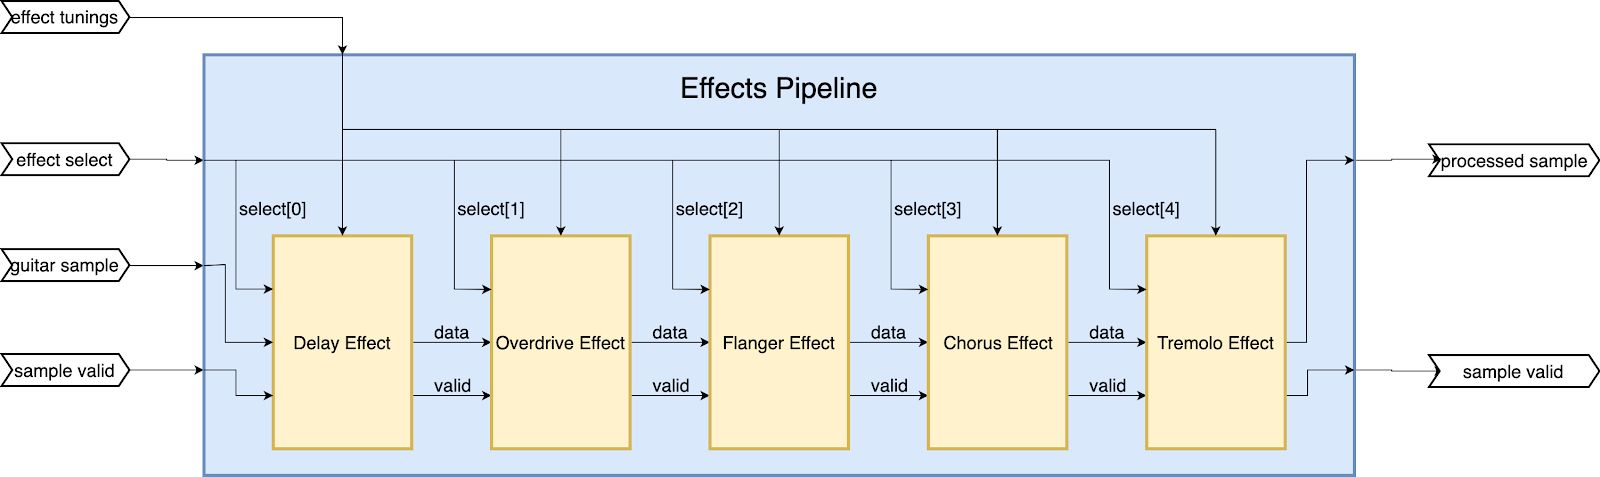
\includegraphics[scale=0.25]{img/pipe.jpg}
    \captionsetup{format=plain,justification=centering}
    \caption{Planowana struktura potoku efektów, źródło: \cite{fpga_pedal}}
    \label{effects-pipe}
\end{figure}
\vspace{0.5cm}

Każdy blok posiada trzy standardowe wejścia oraz dwa standardowe wyjścia. Projekt zakłada wykorzystanie 16-bitowych próbek dźwięku, co determinuje szerokość szyn danych. Wejścia \verb|valid| aktywowane są zboczem narastajacym i~oznaczają pojawienie się nowej próbki na wejściu bloku. Po przetworzeniu próbki moduł ma obowiązek wystawienia danych na linię wyjściową oraz wygenerowanie zbocza narastającego na wyjściu \verb|valid|, które podłączone jest do odpowiadającego wejścia następnego modułu. Każdy z~bloków posiada także jednobitowe wejście \verb|enable|. Stan niski na tej linii oznacza, że blok powinien przekazywać na swoje wyjście próbkę wejściową bez jej modyfikowania. Każdy blok może dodatkowo implementować arbitralne wejścia konfiguracyjne specyficzne dla działania danego algorytmu. W~przypadku blok \textit{overdrive} może być to na przykład 8-bitowa wartość wzmocnienia sygnału i~16-bitowe wartości górnego i~dolnego nasycenia (szczegóły opisano w~dalszej części dokumentu).

Tak zaprojektowana struktura pozwala w~łatwy sposób modyfikować obecne w~systemie efekty oraz nie nakłada ścisłych ograniczeń na interfejs użytkownika wykorzystywany do ich kontrolowania. Również sposób dostarczania i~odbierania danych z~potoku nie jest dzięki temu ograniczony do konkretnego interfejsu komunikacyjnego.

% ----------------------------------------------------------- Overdive ------------------------------------------------------------- %

\subsection{Overdrive}

Jak nakreślono we wstępie efekt przesterowania (ang. \textit{overdive}) określa zespół metod prowadzących do znacznego zniekształcenia sygnału bazowego poprzez dodanie do niego dodatkowych składowych harmonicznych. Częstym sposobem implementacji takiego efektu jest obustronne przycinanie sygnału wejściowego. W~niniejszym projekcie zastosowana zostanie struktura przedstawiona na Rys. {effects-overdrive}.

\vspace{0.5cm}
\begin{figure}[ht]
    \centering
    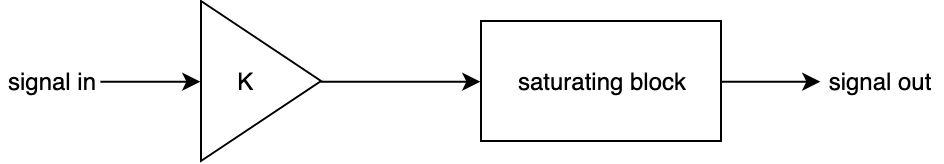
\includegraphics[scale=0.4]{img/overdrive.jpg}
    \captionsetup{format=plain,justification=centering}
    \caption{Schemat bloku \textit{overdrive}, źródło: \cite{fpga_pedal}}
    \label{effects-overdrive}
\end{figure}
\vspace{0.5cm}

Pierwszym etapem przetwarzania jest tutaj wzmocnienie sygnały wejściowego o~wartość kontrolowaną przez rejestr wejsciowy bloku. Zakres potencjalnego wzmocnienia zostanie ustalony na etapie testowania układu. Będzie ono realizowane poprzez 16-bitowe mnożenie z~nasyceniem. Wzmocniony sygnał zostaje następnie przepuszczony przez blok nasycenia. Jeżeli jego wartość mieści się pomiędzy skonfigurowanymi poziomami zostaje on podany na wyjście bez dalszych modyfikacji. W~przeciwnym wypadku na wyjściu pojawia się odpowiednia wartość nasycenia. Funkcjonalność ta może zostać zaimplementowana przy użycia dwóch 16-bitowych komparatorów oraz multipleksera.

% ------------------------------------------------------------ Delay --------------------------------------------------------------- %

\subsection{Delay}

Efekt pogłosu uzyskiwany jest poprzez sumowanie przychodzących próbek z~próbkami opóźnionymi o~określoną liczbę cykli. Realizacja takiego bloku może bazować na filtrze typu FIR (ang. \textit{Finite Impulse Response}) lub IIR (ang. \textit{Infinite Impulse Response}). W~przypadku pierwszego z~nich przeszłe próbki są opóźnionymi wersjami \textbf{sygnału wejściowego}. Liczba próbek sumowanych może być stała lub parametryzowana. Drugi sposób implementacji przewiduje sumowanie pórbki wejściowej jedynie z~jedną wersją opóźnioną sygnału. Wersja ta jest jednak pobierana z~\textbf{wyjścia układu}, co oznacza, że jest ona zależna od wszystkich poprzednich próbek sygnału. Właśnie to rozwiązanie zostanie zastosowane w~niniejszym projekcie. Jego struktura została przedstawiona na Rys.\ref{effects-delay}. W~celu uzyskania stabilnego układu konieczne jest wprowadzenia tłumienia sygnału opóźnionego. Kierując się informacjami zawartymi w~\cite{fpga_pedal} wartości tego tłumienia przyjęto w~zakresie od $0$ do $0.5$. W~celu otrzymania takiego zakresu wyjście z~bloku mnożącego będzie przepusówane o~8~bitów w~prawo (tj. dzielone przez 256).

\vspace{0.5cm}
\begin{figure}[ht]
    \centering
    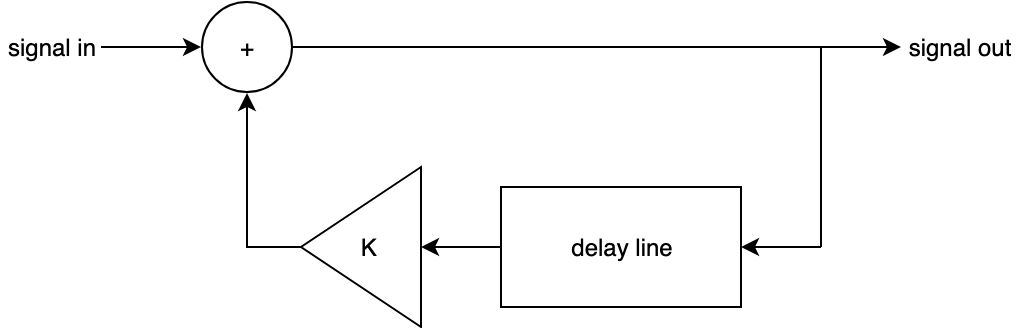
\includegraphics[scale=0.4]{img/delay.jpg}
    \captionsetup{format=plain,justification=centering}
    \caption{Schemat bloku \textit{delay}, źródło: \cite{fpga_pedal}}
    \label{effects-delay}
\end{figure}
\vspace{0.5cm}

Od strony technicznej implementacyja takiego bloku wymaga układu mnożącego, kolejki typu FIFO oraz multipleksera. Siła tłumienia echa ustalana jest poprzez wartość jednego z~wejść do układu mnożącego. Głębokość echa definiuje z~kolei indeks rejestru w~kolejce, którego wartość wystawiana jest na wyjście modułu opóźniającego. Oba parametry efektu regulowane będą przez rejestry wejściowe bloku. Maksymalna głębokość kolejki zostanie ustalona na etapie testowania.

% ----------------------------------------------------------- Flanger -------------------------------------------------------------- %

\subsection{Flanger}

\textit{Flagner} jest efektem, którego brzmienie trudno opisać, jednak zasada jego działania jest stosunkowo prosta. Efekt ten powstaje poprzez nałożenie na sygnał filtru grzebieniowego, którego charakterystyka amplitudowa wykonuje sinusoidalne oscylacje w~okół ustalonego punktu. W~prakyce układ taki realizuje się poprzez sumowanie sygnału z~jego opóźnionymi (nieprzetworzonymi) wersjami. Wartość tego opóźnienia jest jednak okresowo zmienna. Struktura takiego rozwiązania przedstawiona została na Rys.\ref{effects-flanger}. Aby kontrolować siłę efektu do ukłądu wprowadzone zostaną dodatkowe bloki tłumienia. Ich wartość zawierać się będzie w~przedziale od $0$~do $1$, natomiast ich suma będzie stale równa $1$. Podobnie jak w~przypadku pogłosu wykorzystywana głębokość kolejki FIFO (a~tym samym efektywna amplituda oscylacji wartości opóźnienia) będzie ustalana porpzez zewnętrzny parametr.

\vspace{0.5cm}
\begin{figure}[ht]
    \centering
    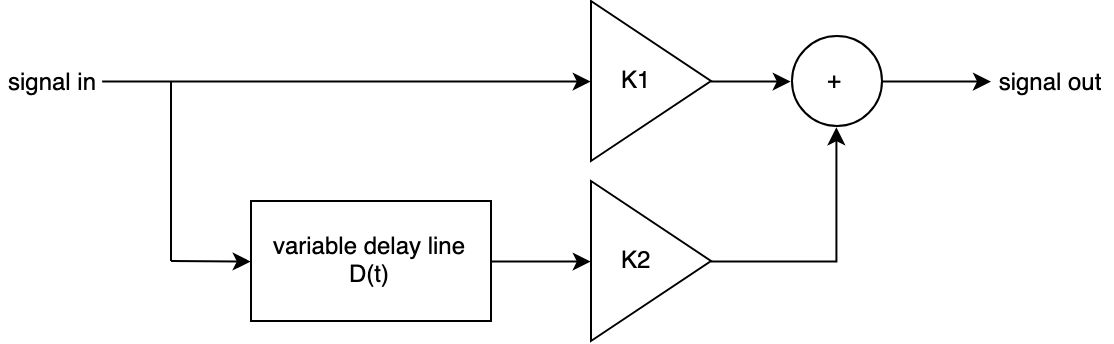
\includegraphics[scale=0.4]{img/flanger.jpg}
    \captionsetup{format=plain,justification=centering}
    \caption{Schemat bloku \textit{flanger}, źródło: \cite{fpga_pedal}}
    \label{effects-flanger}
\end{figure}
\vspace{0.5cm}

Implementacja efektu będzie wykorzystywac bloki stworzone podczas realizacji poprzedniego efektu takie jak układy mnożące oraz kolejka FIFO. Dodatkowym elementem będzie tutaj generator funkcji sinus o~zmiennej częstotliwości. Czestotliwość ta będzie również ustalana poprzez zewnętrzny parametr.

% ----------------------------------------------------------- Tremolo -------------------------------------------------------------- %

\subsection{Tremolo}

Efekt tremolo uzyskuje się poprez modulację amplitudy sygnału wejściowego. Jest to realizowane poprzez mnożenie sygnału z~pewną funkcją okresową jak np. sinus lub fala trójkątna. W~projekcie zaimplementowane zostaną oba rodzaje modulacji. Po wykonaniu testów wybrany zostanie ten, który będzie pozwalał uzyskać ciekawsze brzmienie. Schemat blokowy rozwiązania został przedstawiony na Rys.\ref{effects-tremolo}. Podobnie jak w~przypadku pogłosu wykorzystane zostanie tu 8-bitowe przesówanie wyniku mnożenia celem uzyskania efektywnej amplitudy fali modulującej w~zakresie od $0$ do $1$ (przy załżeniu, że wyjście z~generatora fali ma wartość 8-bitową).

\vspace{0.5cm}
\begin{figure}[ht]
    \centering
    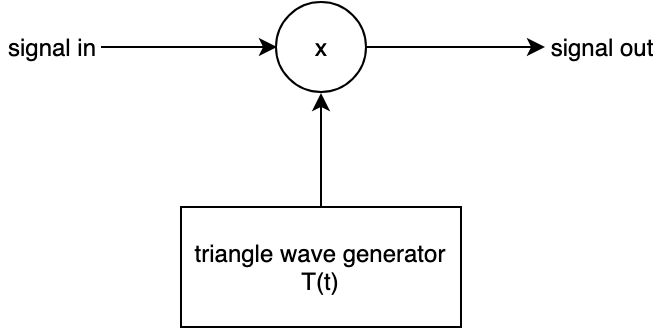
\includegraphics[scale=0.4]{img/tremolo.jpg}
    \captionsetup{format=plain,justification=centering}
    \caption{Schemat bloku \textit{tremolo}, źródło: \cite{fpga_pedal}}
    \label{effects-tremolo}
\end{figure}
\vspace{0.5cm}